\documentclass{beamer}

\mode<presentation>
{
  \usetheme{default}
  \usecolortheme{default}
  \usefonttheme{default}
  \setbeamertemplate{navigation symbols}{}
  \setbeamertemplate{caption}[numbered]
  \setbeamertemplate{footline}[page number]
  \setbeamercolor{frametitle}{fg=white}
  \setbeamercolor{footline}{fg=black}
} 

\usepackage[english]{babel}
\usepackage[utf8x]{inputenc}
\usepackage{tikz}
\usepackage{listings}
\usepackage{courier}
\usepackage{array}
\usepackage{bold-extra}
\usepackage{minted}

\xdefinecolor{darkblue}{rgb}{0.1,0.1,0.7}
\xdefinecolor{darkgreen}{rgb}{0,0.5,0}
\xdefinecolor{darkgrey}{rgb}{0.35,0.35,0.35}
\xdefinecolor{darkorange}{rgb}{0.8,0.5,0}
\xdefinecolor{darkred}{rgb}{0.7,0,0}
\xdefinecolor{dianablue}{rgb}{0.18,0.24,0.31}
\definecolor{commentgreen}{rgb}{0,0.6,0}
\definecolor{stringmauve}{rgb}{0.58,0,0.82}

\lstset{ %
  backgroundcolor=\color{white},      % choose the background color
  basicstyle=\ttfamily\small,         % size of fonts used for the code
  breaklines=true,                    % automatic line breaking only at whitespace
  captionpos=b,                       % sets the caption-position to bottom
  commentstyle=\color{commentgreen},  % comment style
  escapeinside={\%*}{*)},             % if you want to add LaTeX within your code
  keywordstyle=\color{blue},          % keyword style
  stringstyle=\color{stringmauve},    % string literal style
  showstringspaces=false,
  showlines=true
}

\lstdefinelanguage{scala}{
  morekeywords={abstract,case,catch,class,def,%
    do,else,extends,false,final,finally,%
    for,if,implicit,import,match,mixin,%
    new,null,object,override,package,%
    private,protected,requires,return,sealed,%
    super,this,throw,trait,true,try,%
    type,val,var,while,with,yield},
  otherkeywords={=>,<-,<\%,<:,>:,\#,@},
  sensitive=true,
  morecomment=[l]{//},
  morecomment=[n]{/*}{*/},
  morestring=[b]",
  morestring=[b]',
  morestring=[b]"""
}

\title[2017-05-23-ecosystem-dataformats]{Survey of data formats and conversion tools}
\author{Jim Pivarski}
\institute{Princeton University -- DIANA}
\date{May 23, 2017}

\begin{document}

\logo{\pgfputat{\pgfxy(0.11, 8)}{\pgfbox[right,base]{\tikz{\filldraw[fill=dianablue, draw=none] (0 cm, 0 cm) rectangle (50 cm, 1 cm);}}}\pgfputat{\pgfxy(0.11, -0.6)}{\pgfbox[right,base]{\tikz{\filldraw[fill=dianablue, draw=none] (0 cm, 0 cm) rectangle (50 cm, 1 cm);}\includegraphics[height=0.99 cm]{diana-hep-logo.png}\tikz{\filldraw[fill=dianablue, draw=none] (0 cm, 0 cm) rectangle (4.9 cm, 1 cm);}}}}

\begin{frame}
  \titlepage
\end{frame}

\logo{\pgfputat{\pgfxy(0.11, 8)}{\pgfbox[right,base]{\tikz{\filldraw[fill=dianablue, draw=none] (0 cm, 0 cm) rectangle (50 cm, 1 cm);}\includegraphics[height=1 cm]{diana-hep-logo.png}}}}

% Uncomment these lines for an automatically generated outline.
%\begin{frame}{Outline}
%  \tableofcontents
%\end{frame}

%%%%%%%%%%%%%%%%%%%%%%%%%%%%%%%%%%%%%%%%%%%%%%%%%%%%%%%

\begin{frame}{The landscape of generic containers}
\vspace{0.25 cm}
\small By ``generic,'' I mean file formats that define general structures that we can specialize for particular kinds of data, like XML and JSON, but we're interested in binary formats with schemas for efficient numerical storage.

\vspace{0.25 cm}
\mbox{\hspace{-0.75 cm}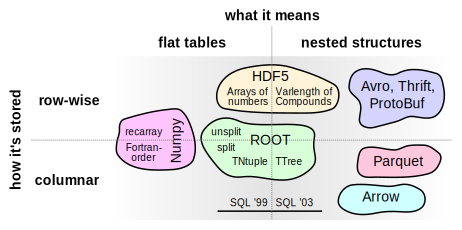
\includegraphics[width=1.15\linewidth]{table-of-formats.pdf}}
\end{frame}

\begin{frame}{The landscape of generic containers}
\vspace{0.5 cm}
\mbox{\hspace{-0.75 cm}\begin{minipage}{1.1\linewidth}
\begin{description}\setlength{\itemsep}{0.15 cm}
\item[ROOT:]<1-> can do anything with the right settings
\item[HDF5:]<2-> stores block-arrays very well, good for flat ntuples; can use variable-length arrays of compounds to store e.g.\ lists of particles, but not in an efficient, columnar way \textcolor{gray}{(?)}
\item[Numpy:]<3-> usually in-memory, but has an efficient file format; only for block-arrays \textcolor{gray}{(can hold Python objects, but not efficiently)}
\item[Avro et al:]<4-> interlingual, binary, deep structures with schemas, row-wise storage is best for streaming and RPC
\item[Parquet:]<5-> extension of Avro et al with {\it columnar} storage, intended for databases and fast querying
\item[Arrow:]<6-> in-memory extension of Parquet \\ intended for zero-copy \\ communication among \\ databases, query servers, \\ analysis frameworks, etc.
\end{description}
\end{minipage}\hspace{-0.75 cm}}

\vspace{-2.5 cm}
\hfill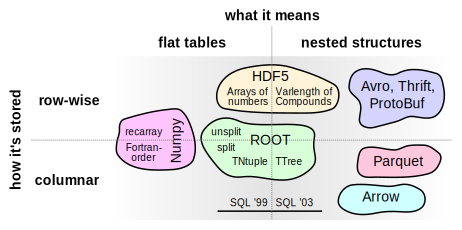
\includegraphics[width=0.5\linewidth]{table-of-formats.pdf}\hspace{-0.9 cm}
\end{frame}

\begin{frame}{Is there a performance penalty?}
\vspace{0.35 cm}
\begin{columns}
\begin{column}{0.55\linewidth}
\begin{itemize}
\item<1-> Formats differ most in how {\it nested} structure is represented:
\small

\vspace{0.1 cm}
\textcolor{darkblue}{Avro:} whole records are contiguous

\textcolor{darkblue}{ROOT:} each leaf is contiguous with list sizes in a separate array

\textcolor{darkblue}{Parquet:} each leaf is contiguous with depth in ``repetition levels''

\normalsize
\item<2-> Nevertheless, differences (with gzip/deflate) are only $\sim$20\%. Use-cases may have more variation than choice of format.

\item<3-> Speed depends more on runtime representation than file format.

\scriptsize
\vspace{0.1 cm}
E.g.\ Avro's C library loads into its custom C objects in 113~sec; Avro's Java library in 8.3~sec! But if Avro's C library reads through the same row-wise data and fills {\it minimalist} objects, it's 5.4~sec.

\end{itemize}
\end{column}
\uncover<2->{\vrule{}}
\begin{column}{0.5\linewidth}
\begin{onlyenv}<1>
\begin{center}
\includegraphics[width=0.5\linewidth]{columnar.png}
\end{center}
\vspace{1 cm}
\end{onlyenv}
\begin{onlyenv}<2->
\begin{center}
\begin{minipage}{0.9\linewidth}
\scriptsize 47\,407 $t\bar{t}$ Monte Carlo events in {\tt TClonesArrays} or variable-length lists of custom classes.

\vspace{0.1 cm}
ROOT 6.06, Avro 1.8.1, Parquet 1.8.1.
\end{minipage}

\vspace{0.25 cm}
\small
\begin{tabular}{l c c}
format         & MB  & rel. \\\hline
ROOT none      & 399 & 1.96 \\
\textcolor{darkblue}{ROOT gzip 1}    & \textcolor{darkblue}{204} & \textcolor{darkblue}{1.00} \\
ROOT gzip 2    & 208 & 1.02 \\
ROOT gzip 9    & 202 & 0.99 \\\hline
Avro none      & 237 & 1.16 \\
Avro snappy    & 198 & 0.97 \\
\textcolor{darkblue}{Avro deflate}   & \textcolor{darkblue}{180} & \textcolor{darkblue}{0.88} \\
Avro LZMA      & 169 & 0.83 \\\hline
Parquet none   & 210 & 1.03 \\
Parquet snappy & 200 & 0.98 \\
\textcolor{darkblue}{Parquet gzip}   & \textcolor{darkblue}{176} & \textcolor{darkblue}{0.86} \\
\end{tabular}

\vspace{0.25 cm}
\scriptsize I don't have a grand study of all formats.
\end{center}
\end{onlyenv}
\end{column}
\end{columns}
\end{frame}

\begin{frame}{What matters is what you'll use it with}
\vspace{0.5 cm}
\begin{center}
\renewcommand{\arraystretch}{1.3}
\begin{tabular}{r p{0.7\linewidth}}
\textcolor{darkblue}{ROOT} & is the best way to access petabytes of \only<1>{\textcolor{black}{\mbox{HEP data}}}\only<2>{\textcolor{red}{\underline{HEP data}}} and use tools developed in HEP \\\hline
\textcolor{darkblue}{HDF5} & is the best way to use tools developed in \only<1>{\textcolor{black}{\mbox{other sciences}}}\only<2>{\textcolor{red}{\underline{other sciences}}}, particuarly R, MATLAB, HPC \\\hline
\textcolor{darkblue}{Numpy} & is the best way to use the scientific Python ecosystem, particularly recent \only<1>{\textcolor{black}{\mbox{machine learning}}}\only<2>{\textcolor{red}{\underline{machine learning}}} software \\\hline
\textcolor{darkblue}{Avro et al} & is the best way to use the \only<1>{\textcolor{black}{\mbox{Hadoop ecosystem}}}\only<2>{\textcolor{red}{\underline{Hadoop ecosystem}}}, particularly streaming frameworks like Storm \\\hline
\textcolor{darkblue}{Parquet} & is the best way to use \only<1>{\textcolor{black}{\mbox{database-like}}}\only<2>{\textcolor{red}{\underline{database-like}}} tools in the Hadoop ecosystem, such as SparkSQL \\\hline
\textcolor{darkblue}{Arrow} & is in its infancy, but is already a good way to \only<1>{\textcolor{black}{\mbox{share data}}}\only<2>{\textcolor{red}{\underline{share data}}} between Python (Pandas) DataFrames and R DataFrames \\
\end{tabular}
\end{center}
\end{frame}

\begin{frame}{Conversions: getting from here to there}
\vspace{0.5 cm}
\mbox{\hspace{-0.75 cm}\only<1>{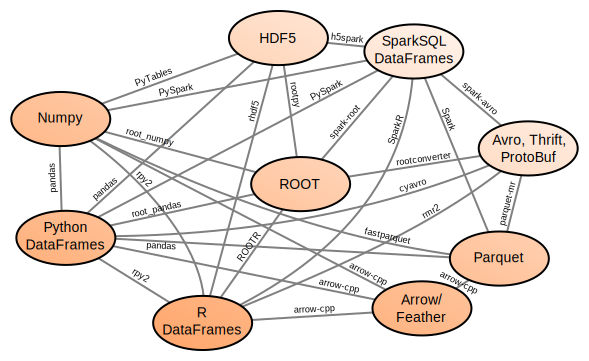
\includegraphics[width=1.15\linewidth]{conversions3.pdf}}\only<2>{\includegraphics[width=1.15\linewidth]{conversions4.pdf}}\only<3>{\includegraphics[width=1.15\linewidth]{conversions5.pdf}}\only<4>{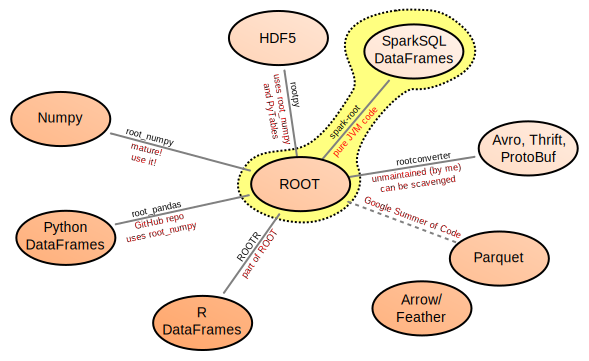
\includegraphics[width=1.15\linewidth]{conversions6.pdf}}}
\end{frame}

\begin{frame}[fragile]{ROOT is now a Spark DataFrame}
\vspace{0.5 cm}
Launch Spark with JARs from Maven Central (zero install).

\vspace{-0.05 cm}
\footnotesize
\begin{minted}{bash}
pyspark --packages org.diana-hep:spark-root_2.11:0.1.11
\end{minted}

\normalsize
\vspace{0.25 cm}
Read ROOT files as you would any other DataFrame.

\footnotesize
\begin{minted}{python}
df = sqlContext.read \
       .format("org.dianahep.sparkroot") \
       .load("hdfs://path/to/files/*.root")
\end{minted}

\begin{verbatim}
df.printSchema()
root
 |-- met: float (nullable = false)
 |-- muons: array (nullable = false)
 |    |-- element: struct (containsNull = false)
 |    |    |-- pt: float (nullable = false)
 |    |    |-- eta: float (nullable = false)
 |    |    |-- phi: float (nullable = false)
 |-- jets: array (nullable = false)
 |    |-- element: struct (containsNull = false)
 |    |    |-- pt: float (nullable = false)
\end{verbatim}
\end{frame}

\begin{frame}{}

\only<1-2>{{\mbox{\hspace{-1 cm}\includegraphics[width=1.2\linewidth]{rootio-screenshot.png}}}}
\only<3-4>{{\mbox{\hspace{-1 cm}\includegraphics[width=1.2\linewidth]{root4j.png}}}}

\begin{onlyenv}<2>
\vspace{-6.2 cm}\hfill\begin{minipage}{3 cm}
\begin{center}
\mbox{\begin{minipage}{2.3 cm}
\centering \includegraphics[width=2 cm]{tonyJohnson_new.jpg}

\centering Tony Johnson

\centering SLAC
\end{minipage}\hspace{-3.2 cm}}
\end{center}
\end{minipage}\hspace{1 cm}\vspace{3.5 cm}
\end{onlyenv}
\begin{onlyenv}<4>
\vspace{-3.5 cm}\hfill\begin{minipage}{3 cm}
\begin{center}
\includegraphics[width=2 cm]{viktor.jpg}

Viktor Khristenko

{\small University of Iowa}
\end{center}
\end{minipage}\hspace{1 cm}\vspace{3.5 cm}
\end{onlyenv}

\end{frame}









%% \begin{frame}[fragile]{root\_numpy: mature! use it!}
%% \begin{center}
%% \textcolor{blue}{\underline{\url{http://scikit-hep.org/root_numpy}}}
%% \end{center}

%% \footnotesize
%% \begin{minted}{python}
%% import root_numpy

%% # get an array from a ROOT file named by string
%% filename = root_numpy.testdata.get_filepath("test.root")
%% array1 = root_numpy.root2array(filename, "tree")

%% # or get an array from a PyROOT TFile/TTree
%% import ROOT
%% rootfile = ROOT.TFile(filename)
%% roottree = rootfile.Get("tree")
%% array2 = root_numpy.tree2array(roottree)
%% \end{minted}

%% \vspace{0.5 cm}
%% {\normalsize Use {\tt TTree::Draw} syntax to transform branches and cut events.}

%% \begin{minted}{python}
%% array3 = root_numpy.tree2array(roottree,
%%     branches=["x", "y", "sqrt(y)", "TMath::Landau(x)"],
%%     selection="z > 0")
%% \end{minted}
%% \end{frame}

%% \begin{frame}[fragile]{c2numpy: used in a handful of projects}
%% \vspace{0.5 cm}
%% Pure-header C library: drop it in and write Numpy files.

%% \begin{center}
%% \textcolor{blue}{\underline{\url{https://github.com/diana-hep/c2numpy}}}
%% \end{center}

%% \scriptsize
%% \begin{minted}{c++}
%% #include "c2numpy.h"

%% c2numpy_init(&writer, "output/tracks", 1000);
%% c2numpy_addcolumn(&writer, "pt", C2NUMPY_FLOAT64);
%% c2numpy_addcolumn(&writer, "eta", C2NUMPY_FLOAT64);
%% c2numpy_addcolumn(&writer, "phi", C2NUMPY_FLOAT64);

%% ...

%% for (auto track = tracks->cbegin();
%%      track != tracks->end();
%%      ++track) {
%%   c2numpy_float64(&writer, track->pt());
%%   c2numpy_float64(&writer, track->eta());
%%   c2numpy_float64(&writer, track->phi());
%% }
%% \end{minted}
%% \end{frame}

%% \begin{frame}{Zero-copy between CMSSW and Numpy}
%% \vspace{0.5 cm}
%% First demonstration last week; may become a common tool.

%% \begin{center}
%% \textcolor{blue}{\tt c2numpy/commonblock}
%% \end{center}

%% \includegraphics[width=\linewidth]{direct-memory.png}
%% \end{frame}

\end{document}
